\subsection{Introduction to Distributed Matrices}
\makesubcontentsslidessec


\begin{frame}
  \begin{block}{Distributed Matrices}\pause
  Most problems in data science are matrix algebra problems, so:
  \begin{center}
  $\text{Distributed matrices} \implies \text{Handle Bigger data}$
  \end{center}
  \end{block}
\end{frame}


% \begin{frame}[fragile]
%   \begin{block}{Distributed Matrices}\pause
%   High level OOP allows \emph{native} serial R syntax:
%   \begin{lstlisting}
% x <- x[-1, 2:5]
% x <- log(abs(x) + 1)
% xtx <- t(x) %*% x
% ans <- svd(solve(xtx))
%   \end{lstlisting}
%   \vspace{.4cm}
%   However\dots
%   \end{block}
% \end{frame}
% 
% 
% \begin{frame}
%   \begin{block}{Distributed Matrices}\pause
%   ddmatrix:
%     \begin{itemize}
%      \item \textbf{D}istributed \textbf{MAT}rix data structure.
%      \item No single processor should hold all of the data.
%      \item Block-cyclic matrix distributed across a 2-dimensional grid of processors.
%      \item Very robust, but confusing data structure.
%     \end{itemize}
%   \end{block}
% \end{frame}



\begin{frame}
\begin{block}{Distributed Matrices}
\begin{figure}[ht]
        \centering
        \begin{subfigure}[b]{0.3\textwidth}
                \centering
\includegraphics[height=5cm,width=\textwidth]%
{../common/pics/dmat/dmat_block}
                \caption{Block}
        \end{subfigure}
        \hspace{.1cm}
        \begin{subfigure}[b]{0.3\textwidth}
                \centering
                
\includegraphics[height=5cm,width=\textwidth]%
{../common/pics/dmat/dmat_cyclic}
                \caption{Cyclic}
        \end{subfigure}
        \hspace{.01cm}
        \begin{subfigure}[b]{0.3\textwidth}
                \centering
                
\includegraphics[height=5cm,width=\textwidth]%
{../common/pics/dmat/dmat_blockcyclic}
                \caption{Block-Cyclic}
        \end{subfigure}
        \caption{Matrix Distribution Schemes}\label{fig:dmat1d}
\end{figure}
\end{block}
\end{frame}



\begin{frame}
\begin{block}{Distributed Matrices}
\begin{figure}[ht]
        \centering
        \begin{subfigure}[b]{0.3\textwidth}
                \centering
                
\includegraphics[height=5cm,width=\textwidth]%
{../common/pics/dmat/dmat_block2d}
                \caption{2d Block}
        \end{subfigure}%
        \hspace{.1cm}
        \begin{subfigure}[b]{0.3\textwidth}
                \centering
                
\includegraphics[height=5cm,width=\textwidth]%
{../common/pics/dmat/dmat_cyclic2d}
                \caption{2d Cyclic}
        \end{subfigure}
        \hspace{.01cm}
        \begin{subfigure}[b]{0.3\textwidth}
                \centering
                
\includegraphics[height=5cm,width=\textwidth]%
{../common/pics/dmat/dmat_blockcyclic2d}
                \caption{2d Block-Cyclic}
        \end{subfigure}
        \caption{Matrix Distribution Schemes Onto a 2-Dimensional 
Grid}\label{fig:dmat2d}
\end{figure}
\end{block}
\end{frame}



\begin{frame}
\begin{block}{Processor Grid Shapes}
\begin{table}[ht]
        \centering
        \begin{subfigure}[b]{0.23\textwidth}
                \centering
              $\left[\begin{tabular}{l}
                  0 \\ 1 \\ 2 \\ 3 \\ 4 \\ 5
                \end{tabular}\right]^T$
                \caption{$1\times 6$}
        \end{subfigure}
        \begin{subfigure}[b]{0.23\textwidth}
                \centering
                $\left[\begin{tabular}{lll}
                  0 & 1 & 2\\
                  3 & 4 & 5
                \end{tabular}\right]$
                \caption{$2\times 3$}
        \end{subfigure}%
        \begin{subfigure}[b]{0.23\textwidth}
                \centering
              $\left[\begin{tabular}{ll}
                  0 & 1 \\
                  2 & 3\\
                  4 & 5
                \end{tabular}\right]$
                \caption{$3\times 2$}
        \end{subfigure}
        \begin{subfigure}[b]{0.23\textwidth}
                \centering
              $\left[\begin{tabular}{l}
                  0 \\ 1 \\ 2 \\ 3 \\ 4 \\ 5
                \end{tabular}\right]$
                \caption{$6\times 1$}
        \end{subfigure}
        \caption{Processor Grid Shapes with 6 Processors}\label{fig:gridshapes}
\end{table}
\end{block}
\end{frame}





% \begin{frame}
%   \begin{block}{Distributed Matrices}\pause
%   The data structure is a special R class (in the OOP sense) called 
% \code{ddmatrix}.  It is the ``under the rug'' storage for a block-cyclic matrix 
% distributed onto a 2-dimensional processor grid.\\[.4cm]
% {\tiny
% \begin{align*}
% \hspace{.1cm}\text{\code{ddmatrix}}&=\begin{cases}
%  $\textbf{Data}$ & $S4 local submatrix, an R matrix$\\
%  $\textbf{dim}$ & $S4 dimension of the global matrix, a numeric pair$\\
%  $\textbf{ldim}$ & $S4 dimension of the local submatrix, a numeric pair$\\
%  $\textbf{bldim}$ & $S4 ScaLAPACK blocking factor, a numeric pair$\\
%  $\textbf{CTXT}$ & $S4 BLACS context, an numeric singleton$
%  \end{cases}
% \end{align*}
% }with prototype{\tiny
% \begin{align*}
% \hspace{-2.9cm}\text{\code{new("ddmatrix")}}&=\begin{cases}
%  $\textbf{Data}$ & =\text{\code{matrix(0.0)}}\\
%  $\textbf{dim}$ & =\text{\code{c(1,1)}}\\
%  $\textbf{ldim}$ & =\text{\code{c(1,1)}}\\
%  $\textbf{bldim}$ & =\text{\code{c(1,1)}}\\
%  $\textbf{CTXT}$ & =\text{\code{0.0}}
%  \end{cases}
% \end{align*}
% }
%   \end{block}
% \end{frame}


% \begin{frame}
%   \begin{block}{Distributed Matrices:  The Data Structure}\pause
%       Example:  an $9\times 9$ matrix is distributed with a ``block-cycling'' 
% factor of $2\times 2$ on a $2\times 2$ processor grid:
%       \begin{center}
%       \begin{minipage}{.45\textwidth}
%       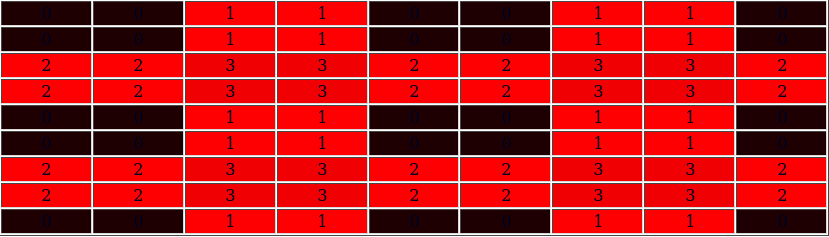
\includegraphics[width=5cm, height=4cm]{../common/pics/dmat/dmat_dist}  
%       \end{minipage}\hspace{.1cm}
%       \begin{minipage}{.45\textwidth}
%       \begin{center}
%       \begin{align*}
%         &=\begin{cases}
%         $\textbf{Data}$ & =\text{\code{matrix(\dots)}}\\
%         $\textbf{dim}$ & =\text{\code{c(9, 9)}}\\
%         $\textbf{ldim}$ & =\text{\code{c(\dots)}}\\
%         $\textbf{bldim}$ & =\text{\code{c(2, 2)}}\\
%         $\textbf{CTXT}$ & =0
%         \end{cases}
%         \end{align*}
%       \end{center}
%       \end{minipage}
%       \end{center}
%     {\small See \url{http://acts.nersc.gov/scalapack/hands-on/datadist.html}}
%   \end{block}
% \end{frame}
